\subsubsection{Constructing the model}
In the model construction, different parameters were tested. At the end, the parameters (and hyper parameters) that yielded the best results are:
\begin{itemize}
    \item number of units: 200, 100 and 50
    \begin{itemize}
        \item In the first layer, we do start with 200 units. As we progress, number of units is decreased in each hidden layer. This results in H1 being 200, H2 100 and H3 has only 50 units. In the last (output) layer, we only have 5 units (since ratings are 1-5).
    \end{itemize}
    
    \item batch size: 128
    \begin{itemize}
        \item Batch size of 64 was the starter and it was tested up to 256. After the batch size of 158, difference was minimal therefore this was the chosen number.
    \end{itemize}
    
    \item number of epochs: 100
    \begin{itemize}
        \item For testing purposes, we have started with 20 epochs to save the time, but went with 100 for final product since the results are better with it.
    \end{itemize}
    
    \item learning rate: 0.00001
    \begin{itemize}
        \item Learning rates of 0.001, 0.0001, 0.00001 and 0.000001 were tested. At the end, 0.00001 gave the best results.
    \end{itemize}
    
    \item momentum
    \begin{itemize}
        \item This function is left disabled. After testing it, momentum of 0.2 and 0.3 brings the best results but if it is disabled (set to 0.0), results are even better.
    \end{itemize}
    
    \item dropout: 0.3 and 0.2
    \begin{itemize}
        \item First layer is using dropout of 0.3. After that, we have decreased dropout to 0.2 for the rest of hidden layers (H2 and H3).
    \end{itemize}
    
    \item activation function: LeakyReLU and softplus in last
    \begin{itemize}
        \item Input function and  hidden layers 1-3 (H1, H2 and H3) are using linear activation function. In the last layer, softplus converts vector to a distribution that can be used for predicting Ratings.
    \end{itemize}
    
    \item number of layers: 5
    \begin{itemize}
        \item Input layer
        \item Hidden layer 1
        \item Hidden layer 2
        \item Hidden layer 3
        \item Output layer
    \end{itemize}
    
    \item optimizer: RMSprop
    \begin{itemize}
        \item Diferent optimises were tested along the way. At the end, there were two candidates: RMSprop and SGD. After some testing RMSprop delivered slightly better results therefore it was chosen.
    \end{itemize}
    
    \item loss function: categorical crossentropy
    \begin{itemize}
        \item Loss function of choice is categorical crossentropy. This is due to our problem being predicting Ratings, therefore we have chosen that.
    \end{itemize}
    
    \item metrics: accuracy
    \begin{itemize}
        \item accuracy is not the only metrics used in industry, but it is the most well known. This is the reason for implementing it. Besides that, confusion matrix is being used as well (that is showcased at the end).
    \end{itemize}
    
\end{itemize}
\tikzset{%
   neuron missing/.style={
    draw=none, 
    scale=4,
    text height=0.333cm,
    execute at begin node=\color{black}$\vdots$
  },
}

\begin{figure}[H]
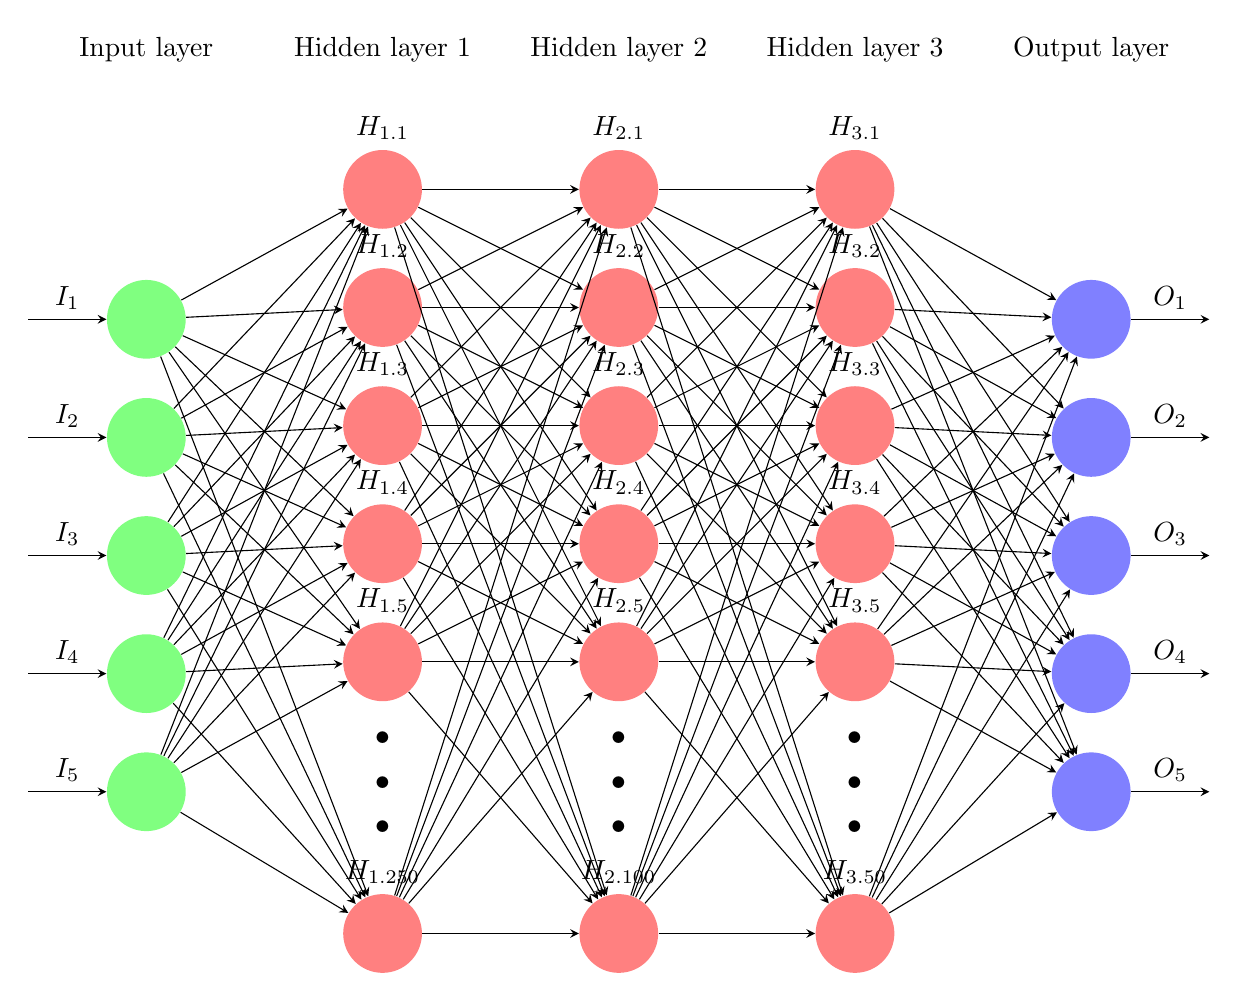
\begin{tikzpicture}[x=1.5cm, y=1.5cm, >=stealth]
%=========================================================================================================
% Input layer
%=========================================================================================================

%First 3 nodes drawn in input layer
\foreach \m/\l [count=\y] in {1,...,5}
{
 \node [circle,fill=green!50,minimum size=1cm] (input-\m) at (0,0.9-\y) {};
}

%Name the input node with 1-256 with the I_1 - I_256, with the arrow coming in
\foreach \l [count=\i] in {1,...,5}
  \draw [<-] (input-\i) -- ++(-1,0)
    node [above, midway] {$I_{\l}$};

%=========================================================================================================
% Hidden layer - 1
%=========================================================================================================
 
%First node drawn in hidden layer
\foreach \m [count=\y] in {1,...,5}
  \node [circle,fill=red!50,minimum size=1cm ] (hidden1-\m) at (2,2-\y) {};
  
% %Last node drawn in hidden layer
 \foreach \m [count=\y] in {6}
   \node [circle,fill=red!50,minimum size=1cm ] (hidden1-\m) at (2,-4.3-\y) {};

%3 dots marked in hidden layer  
 \node [neuron missing]  at (2,-4) {};

% %Name the hidden layer nodes 1-16 as H_1 - H16 above the node
 \foreach \l [count=\i] in {1,...,5,250}
   \node [above] at (hidden1-\i.north) {$H_{1.\l}$};

%=========================================================================================================
% Hidden layer - 2
%=========================================================================================================

%First node drawn in hidden layer
\foreach \m [count=\y] in {1,...,5}
  \node [circle,fill=red!50,minimum size=1cm ] (hidden2-\m) at (4,2-\y) {};
  
% %Last node drawn in hidden layer
 \foreach \m [count=\y] in {6}
   \node [circle,fill=red!50,minimum size=1cm ] (hidden2-\m) at (4,-4.3-\y) {};

%3 dots marked in hidden layer  
 \node [neuron missing]  at (4,-4) {};

% %Name the hidden layer nodes 1-16 as H_1 - H16 above the node
 \foreach \l [count=\i] in {1,...,5,100}
   \node [above] at (hidden2-\i.north) {$H_{2.\l}$};
   
%=========================================================================================================
% Hidden layer - 3
%=========================================================================================================

%First node drawn in hidden layer
\foreach \m [count=\y] in {1,...,5}
  \node [circle,fill=red!50,minimum size=1cm ] (hidden3-\m) at (6,2-\y) {};
  
% %Last node drawn in hidden layer
 \foreach \m [count=\y] in {6}
   \node [circle,fill=red!50,minimum size=1cm ] (hidden3-\m) at (6,-4.3-\y) {};

%3 dots marked in hidden layer  
 \node [neuron missing]  at (6,-4) {};

% %Name the hidden layer nodes 1-16 as H_1 - H16 above the node
 \foreach \l [count=\i] in {1,...,5,50}
   \node [above] at (hidden3-\i.north) {$H_{3.\l}$};   

   
%=========================================================================================================
% Output layer
%=========================================================================================================

%First node drawn in output layer
%\foreach \m [count=\y] in {1}
%  \node [circle,fill=blue!50,minimum size=1cm ] (output-\m) at (8,-1-\y) {};

%Name the output layer nodes 1-16 as O_1 - O_16 with the arrows going out
%\foreach \l [count=\i] in {1}
%  \draw [->] (output-\i) -- ++(1,0)
%    node [above, midway] {$O_{ \l}$};

\foreach \m [count=\y] in {1,...,5}
  \node [circle,fill=blue!50,minimum size=1cm ] (output-\m) at (8,0.9-\y) {};
  
\foreach \l [count=\i] in {1,...,5}
  \draw [->] (output-\i) -- ++(1,0)
    node [above, midway] at (output-\i.north) {$O_{\l}$}; 

%=========================================================================================================
% Draw connections
%=========================================================================================================
%Connections between input layer and hidden layer
\foreach \i in {1,...,5}
  \foreach \j in {1,...,6}
    \draw [->] (input-\i) -- (hidden1-\j);
    
\foreach \i in {1,...,6}
  \foreach \j in {1,...,6}
    \draw [->] (hidden1-\i) -- (hidden2-\j);

\foreach \i in {1,...,6}
  \foreach \j in {1,...,6}
    \draw [->] (hidden2-\i) -- (hidden3-\j);    
    
%\foreach \i in {1,...,6}
%  \foreach \j in {1,...,1}
%    \draw [->] (hidden2-\i) -- (hidden3-\j);

%Connections between hidden layer and output layer
\foreach \i in {1,...,6}
  \foreach \j in {1,...,5}
    \draw [->] (hidden3-\i) -- (output-\j);

%=========================================================================================================
% Draw headers
%=========================================================================================================
%headers
\foreach \l [count=\x from 0] in {Input layer, Hidden layer 1, Hidden layer 2, Hidden layer 3, Output layer}
  \node [align=center, above] at (\x*2,2) {\l};

\end{tikzpicture}
\caption{Visualisation of the model}
\end{figure}
Code block representing how model is build together.
\begin{lstlisting}[language=Python, caption=Build model]
model = models.Sequential()
# hidden layer 1
model.add(layers.Dense(250, 
                       activation='LeakyReLU', 
                       input_dim=X_train.shape[1], 
                       kernel_regularizer=regularizers.l2(0.00001)))
model.add(layers.Dropout(0.3))
# hidden layer 2
model.add(layers.Dense(100, activation='LeakyReLU'))
model.add(layers.Dropout(0.2))
# hidden layer 3
model.add(layers.Dense(50, activation='LeakyReLU'))
model.add(layers.Dropout(0.2))
# output layer, 5 untis since ratings are 1,2,3,4,5
model.add(layers.Dense(5, activation='softplus'))
\end{lstlisting}
Representation of compiling the model.
\begin{lstlisting}[language=Python, caption=Compile model]
model.compile(optimizer='RMSprop', 
              loss='categorical_crossentropy',
              metrics=['accuracy'])
\end{lstlisting}
Fitting the model and saving results into local variable named history.
\begin{lstlisting}[language=Python, caption=Fit model]
history = model.fit(X_train_transf, 
                    y_train_cat, 
                    validation_data=(X_val_transf, y_val_cat),
                    batch_size=158, 
                    epochs=100, 
                    verbose=2)
\end{lstlisting}